\chapter{Phonon induced band gap in graphene \label{chap:kek}}

\section{Theory}
The $\bm{K}$ point Kekul\'e phonon corresponds to a high spatial frequency deformation of graphene's lattice.
Displacement vectors describe the eigenmode of this phonon by detailing the displacements of the atoms in the A and B sub-lattices originally at position $\vec{r}_{A,B}$
\begin{equation}
	u^{A,B}(\vec{r}_{A,B},t)=\frac{1}{2} c \ e^{i \vec{r}_{A,B} \cdot \bm{K}} e^{-i \omega t} 
		\left( \begin{array}{c}
			1 \\
			\mp i
		\end{array} \right)
	 + \text{c.c.} \label{eq:kek:displacements} \ ,
\end{equation}
where the top sign corresponds to the A sub-lattice and the bottom sign corresponds to the B sub-lattice.
Here c is the amplitude, $\omega$ is the frequency of the phonon, and $t$ is time.
Snapshots showing the time dependence of the resulting lattice distortion are shown in Figure \ref{fig:kek:snapshots}.
This phonon mode is special in that the atoms in each sub-lattice rotate around their equilibrium positions without ever returning to equilibrium.
Atoms in the A sub-lattice are left handed, rotating in the clockwise direction while the atoms in the B sub-lattice are right handed.
As time progresses, adjacent A and B sub-lattice atoms dimerize in a sequential fashion.
At $\omega t=\{90 \text{\textdegree}, 210 \text{\textdegree}, 330 \text{\textdegree} \}$ the dimerization switches between the three nearest neighbors.
At all other time the system is in varying phases of dimerization.
This dimerization is similar to the Peierls distortion in polyacetylene except that in this two dimensional analog the system does not gap spontaneously.
Instead the phonon must be continuously excited to maintain the gap.

\begin{figure}
	\begin{center}
	{
% Sizing constants
\newcommand{\alat}{1}
\newcommand{\amp}{.25}
\newcommand{\psize}{1 mm}
\newcommand{\sqth}{1.73205080757}

% Functions which draws the Kekule lattice
\newcommand{\kekdraw}[2]{
	\begin{scope}[xshift=#1*3.5 cm,yshift=-#2*3.5cm,scale=.4]

		%This scope is clipped to limit the drawn lattice to a square
		\clip (-3cm,-3cm) rectangle(3cm,3 cm);
		
		% Cycle through the lattice points
		\foreach \ip in {-2,-1,...,2}
			\foreach \im in {-2,-1,...,2}
			{
			% Draw the unkekuled lattice
			\node at ($\ip*\sqth*\alat/2*(1,{\sqth})+\im*\sqth*\alat/2*(-1,{\sqth})+(0,+\alat/2)$) [Au] {};
			\node at ($\ip*\sqth*\alat/2*(1,{\sqth})+\im*\sqth*\alat/2*(-1,{\sqth})+(0,-\alat/2)$) [Bu] {};

			% Draw the Kekuled lattice
			\node at ($\ip*\sqth*\alat/2*(1,{\sqth})+\im*\sqth*\alat/2*(-1,{\sqth})+(0,+\alat/2)
				+\amp*({cos(120*(\ip-\im)-30*(#1+1+3*#2))},{+sin(120*(\ip-\im)-30*(#1+1+3*#2))} )$)            [A] {};
			\node at ($\ip*\sqth*\alat/2*(1,{\sqth})+\im*\sqth*\alat/2*(-1,{\sqth})+(0,-\alat/2)
				+\amp*({cos(120*(\ip-\im)-30*(#1+1+3*#2))},{-sin(120*(\ip-\im)-30*(#1+1+3*#2))} )$)            [B] {};
			}

	\end{scope}
}

\begin{tikzpicture}[>=stealth,
		Bu/.style={circle,draw=blue!25,fill=blue!10,
			thick,minimum size=\psize,inner sep=0pt}, 					% Unkekuled A sublattice dots
		Au/.style={circle,draw=orange!35,fill=orange!20,
			thick,minimum size=\psize,inner sep=0pt},					% Unkekuled B sublattice dots
		B/.style={circle,draw=blue!50,fill=blue!20,
			thick,minimum size=\psize,inner sep=0pt}, 					% Kekuled A sublattice dots
		A/.style={circle,draw=orange!70,fill=orange!40,
			thick,minimum size=\psize,inner sep=0pt}]					% Kekuled B sublattice dots
		
		\foreach \itc in {-1,0,1}
			\foreach \itr in {0,1,...,3}
			{
				\kekdraw{\itc}{\itr}
				\pgfmathsetmacro\result{30*(\itc+1+3*\itr)};
				\node at (\itc*3.5 cm,-\itr*3.5cm+1.5cm) {$\omega t$=\pgfmathprintnumber[int trunc]{\result}};
			}
\end{tikzpicture}
}
	\end{center}
	\caption[Snapshots of the Kekul\'e phonon mode]{\label{fig:kek:snapshots}
		Snapshots of the Kekul\'e phonon mode spanning one period of oscillation.
		The A sub-lattice is in orange and the B sub-lattice in blue.
		Faded dots indicating the intrinsic graphene lattice are included for reference.}
\end{figure}

The time reversed pair of the $\bm{K}$ Kekul\'e phonon, the $\bm{K'}$ Kekul\'e phonon, corresponds to sub-lattices rotating with opposite handedness.
If both $\bm{K}$ and $\bm{K'}$ modes were excited at once, the rotations with opposite circular polarizations would sum resulting in linear polarized atomic motion.
In this case the dimerization would only be temporary.
The atoms would return to their equilibrium positions during their oscillations.
Thus, it is important to excite exclusively the $\bm{K}$ or $\bm{K'}$ phonon to excite gap.
In the experimental section our method of selecting the phonon will be described.
In the theory section, for simplicity we will continue to concentrate on the $\bm{K}$ phonon.
However, the resulting dispersion is the same for either mode. 

When considering how these phonon modes affect the electronic dispersion, we will use the Born-Oppenheimer approximation.
According to this approximation, the very fast electrons react nearly instantaneously to the slow phonon induced modifications of the lattice.
Thus, the modified electronic dispersion can be calculated assuming the lattice is frozen in sequential snapshots.
In this section this calculation is done using a tight binding model in the expanded unit cell of the deformed lattice.
It is performed in two parts.
First, the effects of the change in lattice periodicity are discussed including a discussion of the zone folded electrical dispersion.
Second, it is shown that by perturbing the zone folded Hamiltonian the phonons gap the electronic dispersion.

\subsection{Kekul\'e geometry}
The Kekul\'e distortion causes an expansion of the unit cell, a reduction of the BZ, and a modification of the primitive lattice vectors and reciprocal lattice vectors.
When referencing this new geometry back to graphene's intrinsic geometry, the notation previously developed in Chapter \ref{chap:TB} is used.
The expanded periodicity of the Kekul\'e lattice is determined by the periodicity of the distortion in Equation \ref{eq:kek:displacements}.
This term repeats whenever 
\begin{equation*}
	2 \pi=\vec{r}_{A,B} \cdot \bm{K}=(m \vec{a}_+ + n \vec{a}_-) \cdot (\vec{b}_+ - \vec{b}_-)/3=\frac{2 \pi}{3} (m-n) \ ,
\end{equation*}
where $m$ and $n$ are integers.
Thus, at any snapshot in time the electrons see the expanded six atom unit cell shown in Figure \ref{fig:kek:geometry}.
This tripled unit cell is time independent; it never returns to the intrinsic two atom basis. 

\begin{figure}
	\begin{center}
	% Comparing the Lattice and BZ with Kekule to without Kekule
{ % Scope so that user defined commands don't carry throughout
% Sizing constants
\newcommand{\alat}{1}
\newcommand{\amp}{.25}
\newcommand{\Klen}{2 cm}
\newcommand{\psize}{2 mm}
\newcommand{\sqth}{1.73205080757}

% Functions which draws the Kekule lattice
\newcommand{\kekdraw}{
	\begin{scope}

		%This scope is clipped to limit the drawn lattice to a square
		\clip (-3.9cm,-4.38cm) rectangle(3.9cm,3cm);
		
		% Cycle through the lattice points
		\foreach \ip in {-3,-2,...,3}
			\foreach \im in {-3,-2,...,3}
			{
			% Draw the unkekuled lattice
			\node at ($\ip*\sqth*\alat/2*(1,{\sqth})+\im*\sqth*\alat/2*(-1,{\sqth})+(0,+\alat/2)$) [Au] {};
			\node at ($\ip*\sqth*\alat/2*(1,{\sqth})+\im*\sqth*\alat/2*(-1,{\sqth})+(0,-\alat/2)$) [Bu] {};

			% Draw the Kekuled lattice
			\node at ($\ip*\sqth*\alat/2*(1,{\sqth})+\im*\sqth*\alat/2*(-1,{\sqth})+(0,+\alat/2)
				+\amp*({cos(120*(\ip-\im)-90)},{+sin(120*(\ip-\im)-90)} )$)            [A] {};
			\node at ($\ip*\sqth*\alat/2*(1,{\sqth})+\im*\sqth*\alat/2*(-1,{\sqth})+(0,-\alat/2)
				+\amp*({cos(120*(\ip-\im)-90)},{-sin(120*(\ip-\im)-90)} )$)            [B] {};
			}

	\end{scope}
}

\begin{tikzpicture}
	% Real space
	\begin{scope}[xshift=-3.75cm, scale=1,>=stealth,
		Bu/.style={circle,draw=blue!25,fill=blue!10,
			thick,minimum size=\psize,inner sep=0pt}, 					% Unkekuled A sublattice dots
		Au/.style={circle,draw=orange!35,fill=orange!20,
			thick,minimum size=\psize,inner sep=0pt},					% Unkekuled B sublattice dots
		B/.style={circle,draw=blue!50,fill=blue!20,
			thick,minimum size=\psize,inner sep=0pt}, 					% Kekuled A sublattice dots
		A/.style={circle,draw=orange!70,fill=orange!40,
			thick,minimum size=\psize,inner sep=0pt},					% Kekuled B sublattice dots
		nnarrow/.style={color=black,very thick, ->}]					% Arrows
		% Draw the lattice
		\kekdraw

		% Draw the primitive lattice vectors
		\draw[nnarrow] (0,-\alat*5/2) -- +( 30:3*\alat)node[anchor=south]{$\vec{A}_+$};
		\draw[nnarrow] (0,-\alat*5/2) -- +(150:3*\alat)node[anchor=south]{$\vec{A}_-$};

		% Draw the unit cell
		\draw[dashed,draw=black!75,rounded corners=.2cm,thick] (-\alat*\sqth*3/4,-\alat*15/4) rectangle (\alat*\sqth*3/4,-\alat*3/4);

	\end{scope}


	% Reciprical space
	\begin{scope}[xshift=3.75cm,yshift=-1 cm,scale=1,
		BZold/.style={color=black!75,very thick,dashed},
		BZnew/.style={color=black,very thick},
		Bar/.style={color=black,very thick,->},
		circ2/.style={radius=1.5pt}]

		% Draw the BZ
		\draw[BZold]
			(  0:\Klen) --
			( 60:\Klen) --
			(120:\Klen) -- 
			(180:\Klen) -- 
			(240:\Klen) -- 
			(300:\Klen) -- 
			(  0:\Klen);

					% Draw the BZ
		\draw[BZnew]
			( 30:\Klen/\sqth) --
			( 90:\Klen/\sqth) --
			(150:\Klen/\sqth) -- 
			(210:\Klen/\sqth) -- 
			(270:\Klen/\sqth) -- 
			(330:\Klen/\sqth) -- 
			( 30:\Klen/\sqth);

		\draw[Bar] (0,0) -- ( 60:\Klen) node[anchor=south west]{$\vec{B}_+$};
		\draw[Bar] (0,0) -- (120:\Klen) node[anchor=south east]{$\vec{B}_-$};

		% Label the high symmetry points
		\draw[fill=black] (0,0) circle[circ2] node[anchor=west]{$\Gamma$};
	\end{scope}
	\node at (-7cm,3.5cm) {\textbf{(a)}};
	\node at ( 1cm,3.5cm) {\textbf{(b)}};
\end{tikzpicture}
}
	\end{center}
	\caption[The geometry of the Kekul\'e lattice]{\label{fig:kek:geometry}
		The real space (a) and reciprocal space (b) geometry of the Kekul\'e lattice.
		(a) shows a snapshot of the atomic positions with the A sub-lattice in orange and the B sub-lattice in blue.	
		For reference, the intrinsic graphene lattice is shown using faded dots.
		The dashed rectangle outlines the time independent unit cell and the labeled arrows represent the primitive lattice vectors.
		In (b) the dashed hexagon indicates the BZ of intrinsic graphene while the hexagon with solid lines indicates the shrunken BZ of the Kekul\'e lattice.
		The primitive reciprocal lattice vectors are labeled along with select high symmetry points.
	}
\end{figure}

The primitive lattice vectors of the Kekule\'e lattice,
\begin{align*}
	\vec{A}_+&=2 \vec{a}_+-\vec{a}_-=\frac{3 a}{2} (+\sqrt{3},1) \\
	\vec{A}_-&=2 \vec{a}_--\vec{a}_+=\frac{3 a}{2} (-\sqrt{3},1) \ ,
\end{align*}
represent a triangular lattice rotated by 90 degrees and expanded by a factor of $\sqrt{3}$ relative to the intrinsic lattice.
This tripling of the area of the unit cell is accompanied by a corresponding decrease in the area of the BZ as shown in Figure \ref{fig:kek:geometry}.
The primitive reciprocal lattice vectors,
\begin{align*}
	\vec{B}_+&=\frac{1}{3} (2\vec{b}_+ + \vec{b}_-)=\frac{2 \pi}{3 \sqrt{3} a}(+1,\sqrt{3}) \\
	\vec{B}_-&=\frac{1}{3} (2\vec{b}_- + \vec{b}_+)=\frac{2 \pi}{3 \sqrt{3} a}(-1,\sqrt{3}) \ ,
\end{align*}
generate a hexagonal BZ rotated 90 degrees and shrunken by a factor of three relative to the intrinsic lattice.
Unlike for intrinsic graphene, the interesting physics occurs near the center of the BZ.
For completeness, three equivalent corners of the BZ are positioned at
\begin{equation*}
	\frac{2 \pi}{9 a} (-\sqrt{3},-1), \ \ \frac{2 \pi}{9 a} (+\sqrt{3},-1), \ \ \textrm{and} \ \  \frac{2 \pi}{9 a} (0,2) \ .
\end{equation*}
Hence, the periodicity of the phonon fully describes the geometry of the expanded lattice.

\subsection{Zone folding}
When the BZ is reduced in size the number of bands in the electronic dispersion is increased.
Energy bands outside the new BZ are folded into the new BZ by translation by reciprocal lattice vectors.
Since the size of BZ is reduced by a factor of three, there are two zone folding schemes resulting in six energy bands.

The zone folding schemes shown in Figure \ref{fig:kek:folding} describe the two distinct ways the symmetry reduced area of the new BZ can be mapped onto via translations of reciprocal lattice vectors.
The rest of the BZ can be constructed using symmetry operations on the symmetry reduced area.
In both zone folding schemes, the Dirac point is translated from the corner of the old BZ to the zone center of the new BZ.
Thus, the $\Gamma$ point is the most interesting point in the new BZ.
It is also worth noting that the right edge of the symmetry reduced area in zone fold 1 shares its right edge with the symmetry reduced area already inside the new BZ.
Also, the top edge of the symmetry reduced area is shared between zone fold 1 and zone fold 2.

\begin{figure}
	\begin{center}
	{
\newcommand{\Klen}{2 cm}
\newcommand{\sqth}{1.73205080757}
\newcommand{\BZ}{
	% Draw the old BZ
	\draw[BZold]
		(  0:\Klen) --
		( 60:\Klen) --
		(120:\Klen) -- 
		(180:\Klen) -- 
		(240:\Klen) -- 
		(300:\Klen) -- 
		(  0:\Klen);

	% Draw the new BZ
	\draw[BZnew]
		( 30:\Klen/\sqth) --
		( 90:\Klen/\sqth) --
		(150:\Klen/\sqth) -- 
		(210:\Klen/\sqth) -- 
		(270:\Klen/\sqth) -- 
		(330:\Klen/\sqth) -- 
		( 30:\Klen/\sqth);
}
\newcommand{\elemone}[2]
{
	\draw[fill=#1!30,draw=#1!90,rotate=#2] (0,0) -- (-30:\Klen/\sqth) -- (30:\Klen/\sqth) --cycle;
	\draw[fill=#1!30,draw=#1!90,rotate=#2,xshift=-\Klen] (0,0) -- (-30:\Klen/\sqth) -- (30:\Klen/\sqth) --cycle;
}

\newcommand{\elemtwo}[3]
{
	\draw[fill=#1!30,draw=#1!90,xscale=#3,rotate=#2]  (0,0) -- (\Klen/2,0) -- (30:\Klen/\sqth) --cycle;
	\draw[fill=#1!30,draw=#1!90,xscale=#3,rotate=#2,shift={(60:-\Klen)}] (0,0) -- (\Klen/2,0) -- (30:\Klen/\sqth) --cycle;
}

\begin{tikzpicture}[scale=1,
		BZnew/.style={color=black!90,thick},
		BZold/.style={color=black!90,thick,dashed},
		Bar/.style={color=black,thick,<-,>=stealth},
		circ2/.style={radius=1.5pt}]

	% Zone fold 1
	\begin{scope}[xshift=-2.5cm]

		% Draws the zones folding in
		\foreach \i/\colora in {0/{red},60/{blue},120/{green},180/{violet},240/{orange},300/{gray}} {
			\elemone{\colora}{\i}
		}

		% Draws on the old and new BZ
		\BZ

		% Draws the reduced symetric elemtn
		\draw[black] (0,0) -- (\Klen/2,0) -- (30:\Klen/\sqth) --cycle;
		\draw[black,xshift=-\Klen] (0,0) -- (\Klen/2,0) -- (30:\Klen/\sqth) --cycle;
		
		% Draws the arrow showing the shift in the reduced element
		\draw[Bar] (15:\Klen/\sqth/2*1.25) --node[above,xshift=.3cm]{$\vec{B}_+-\vec{B}_-$} ++(-\Klen,0);
	\end{scope}

	% Zone fold 2
	\begin{scope}[xshift=+2.5cm]

		% Draws the zones folding in
		\foreach \i/\colora in {0/{red},60/{blue},120/{green},180/{violet},240/{orange},300/{gray}} {
			\elemtwo{\colora}{\i}{1}
		}
		\foreach \i/\colora in {0/{yellow},60/{brown},120/{teal},180/{olive},240/{cyan},300/{magenta}} {
			\elemtwo{\colora}{\i}{-1}
		}

		% Draws on the old and new BZ
		\BZ

		% Draws the reduced symetric elemtn
		\draw[black] (0,0) -- (\Klen/2,0) -- (30:\Klen/\sqth) --cycle;
		\draw[black,shift={(60:-\Klen)}] (0,0) -- (\Klen/2,0) -- (30:\Klen/\sqth) --cycle;
		
		% Draws the arrow showing the shift in the reduced element
		\draw[Bar] ( 15:\Klen/\sqth/2*1.25) -- node[right]{$\vec{B}_+$} ++(240:\Klen);
	\end{scope}

	\node at (-3cm,2.5cm) {\textbf{(a) Zone Fold 1}};
	\node at (2cm,2.5cm) {\textbf{(b) Zone Fold 2}};
\end{tikzpicture}
}
	\end{center}
	\caption[The zone foldings introduced by the Kekul\'e distortion]{\label{fig:kek:folding}
		The zone foldings introduced by the Kekul\'e distortion.
		The outer, dashed hexagon is the BZ of intrinsic graphene and the inner hexagon with solid lines is the new BZ of the Kekul\'e lattice.
		The symmetry reduced area represented by the black outlined triangle is translated into the new BZ by different reciprocal lattice vectors (labeled) for the two folding schemes.
		}
\end{figure}

The hierarchy of the folded energy bands can be determined by comparing the zone folded areas to the electronic dispersion of intrinsic graphene shown in Figure \ref{fig:TB:Dispersion}.
The lowest and highest energy bands will correspond to the unfolded area because the new BZ occupies the basin in the intrinsic graphene dispersion.
Zone fold 1 extends further into the basin of intrinsic graphene's dispersion than zone fold 2 and so gives the second lowest and second highest energy bands.
Finally, the zone fold 2 gives the two middle energy bands.

The zone folded electronic dispersion can either be calculated by folding the dispersion calculated in Chapter \ref{chap:TB} or by performing a tight binding calculation in the expanded unit cell.
Although it is more involved, the tight binding calculation will be done here because it will be needed later.
In this scheme, each of the six atoms in the unit cell must have its own raising and lowering operator.
To simplify this bookkeeping the operators will be referenced back to the three two atom bases which make up the six atom Kekul\'e basis.
These two atom bases are shown in Figure \ref{fig:kek:hoppings}.
The operators $a_{i,l}$ and $b_{i,l}$ are then the lowering operators for the three A sub-lattice atoms and the three B sub-lattice atoms in the lth Kekul\'e basis respectively.
The index $i$ run over the three two atom bases.
In this notation the real space nearest neighbor tight binding Hamiltonian is given by
\newcommand{\rl}[4]{
	a^{\dagger}_{#1,#2} b_{#3,#4}
}
\begin{align}
	H=-\sum_l (
		 & t \rl{1}{l}{1}{l        }+t\rl{1}{l}{2}{l          }+t\rl{1}{l}{3}{l           } \nonumber \\
		+& t \rl{2}{l}{1}{l\uparrow}+t\rl{2}{l}{2}{l          }+t\rl{2}{l}{3}{l\rightarrow} \nonumber \\ 
		+& t \rl{3}{l}{1}{l\uparrow}+t\rl{3}{l}{2}{l\leftarrow}+t\rl{3}{l}{3}{l           } + \text{H.C.} ) \ .
		\label{eq:kek:Hreal}
\end{align}
Later the hopping energies $t$ will be made bond dependent to account for the altered nearest neighbor distances.
In the meantime the bond independent hopping energy of intrinsic graphene, $t_0$, will be used.

\begin{figure}
	\begin{center}
	{
\newcommand{\alat}{1}
\newcommand{\amp}{.075}
\newcommand{\psize}{2 mm}
\newcommand{\sqth}{1.73205080757}

% Functions which draws the Kekule lattice
\newcommand{\kekdraw}{
	\begin{scope}
		% Cycle through the lattice points
		\foreach \ip/\im in {0/0,1/0,0/1,-1/0,0/-1,-1/-1,-1/-2,-2/-1,-2/-2,1/-1,2/-2,1/-2,-1/1,-2/2,-2/1,0/-2,-2/0,-3/0,0/-3,1/-3,-3/1}
			{
			\node at ($\ip*\sqth*\alat/2*(1,{\sqth})+\im*\sqth*\alat/2*(-1,{\sqth})+(0,+\alat/2)
				+\amp*({cos(120*(\ip-\im)-90)},{+sin(120*(\ip-\im)-90)} )$)            [A] {};
			\node at ($\ip*\sqth*\alat/2*(1,{\sqth})+\im*\sqth*\alat/2*(-1,{\sqth})+(0,-\alat/2)
				+\amp*({cos(120*(\ip-\im)-90)},{-sin(120*(\ip-\im)-90)} )$)            [B] {};
			}

	\end{scope}
}
\begin{tikzpicture}[scale=.85,
		B/.style={circle,draw=blue!50,fill=blue!20,
			thick,minimum size=\psize,inner sep=0pt}, 					% Kekuled A sublattice dots
		A/.style={circle,draw=orange!70,fill=orange!40,
			thick,minimum size=\psize,inner sep=0pt},					% Kekuled B sublattice dots
		el1/.style={x radius=.3*\alat,y radius=.85*\alat},				% Style for the ellipse
		hops/.style={thick,black},										% Style for the hopping directions
		nnarrow/.style={color=black, ->,>=stealth}]						% Nearest neighbor vectors

	% Draw the hoppings we work with
	% \ip and \im specify the position of the A unit cell
	% \jp and \jm specify the position of the B unit cell
	\foreach \ip/\im/\jp/\jm in {-1/0/0/0,-1/0/-1/1,-1/0/-1/0,0/-1/0/0,0/-1/1/-1,0/-1/0/-1,-1/-1/-1/0,-1/-1/0/-1,-1/-1/-1/-1}{
		\draw[hops]
			($\ip*\sqth*\alat/2*(1,{\sqth})+\im*\sqth*\alat/2*(-1,{\sqth})+(0,+\alat/2)
			+\amp*({cos(120*(\ip-\im)-90)},{+sin(120*(\ip-\im)-90)} )$) -- 
			($\jp*\sqth*\alat/2*(1,{\sqth})+\jm*\sqth*\alat/2*(-1,{\sqth})+(0,-\alat/2)
			+\amp*({cos(120*(\jp-\jm)-90)},{-sin(120*(\jp-\jm)-90)} )$);
	}

	% Draw the atomic positions
	\kekdraw

	% Draw the Expanded units cells
	\foreach \Api/\Ami in {0/0,1/0,1/1,0/1,-1/0,-1/-1,0/-1}{
		\draw[dashed,draw=black!75,thick,shift={($\Api*3*\alat/2*(\sqth,1)+\Ami*3*\alat/2*(-\sqth,1)$)}]
			(-\alat*\sqth*3/4,-\alat*15/4) rectangle (\alat*\sqth*3/4,-\alat*3/4);
	}

	% Label the Expanded unit cells (only the ones we use)
	\foreach \Api/\Ami/\label in {0/0/$\bm{l}$,1/0/$\bm{l\rightarrow}$,1/1/$\bm{l\uparrow}$,0/1/$\bm{l\leftarrow}$}{
		\node at ($(-\alat*\sqth*3/4,-\alat*15/4)+\Api*3*\alat/2*(\sqth,1)+\Ami*3*\alat/2*(-\sqth,1)$) [anchor=south west] {\label} ;
	}

	% Draw the original unit cells
	% \foreach \api/\ami/\ind in {0/0/1,1/0/2,0/1/3,2/0/3,1/1/1,0/2/2}{
	% 	\draw[dashed,draw=black!75,thick,shift={($\api*\sqth*\alat/2*(1,{\sqth})+\ami*\sqth*\alat/2*(-1,{\sqth})$)}] 
	% 		(0,-3) ellipse[el1] node[xshift=.2cm] {$\bm{\ind}$};
	% }

	\foreach \api/\ami/\ind in {0/0/1,1/0/2,0/1/3,2/0/3,1/1/1,0/2/2}{
		\draw[dashed,draw=black!75,thick,
		shift={($\api*\sqth*\alat/2*(1,{\sqth})+\ami*\sqth*\alat/2*(-1,{\sqth})
				+\amp*({cos(120*(\api-\ami)-90)},0)$)}
		] 
			(0,-3) ellipse[el1] node[xshift=.125cm] {$\bm{\ind}$};

	% Draw the nearest neighbor vectors
	\draw[nnarrow] (6.5cm,-2cm) -- +(270:\alat) node[anchor=north     ]{$\vec{\delta}_1$};
	\draw[nnarrow] (6.5cm,-2cm) -- +( 30:\alat) node[anchor=south west]{$\vec{\delta}_2$};
	\draw[nnarrow] (6.5cm,-2cm) -- +(150:\alat) node[anchor=south east]{$\vec{\delta}_3$};
	}

\end{tikzpicture}
}
	\end{center}
	\caption[Diagram of the hoppings in the expanded Kekul\'e unit cell]{\label{fig:kek:hoppings}
		A diagram of the hoppings included in the Hamiltoninan.
		Hoppings connect atoms originally from the A sub-lattice (orange) to atoms originally from the B sub-lattice (blue).
		They can pass between the labeled intrinsic unit cells (dashed ellipses) and they can also pass between the labeled extended unit cells (dashed rectangles).
		For reference the directions of the nearest neighbor vectors are included.
	}
\end{figure}

Similarly to intrinsic graphene, the individual terms in the sum can be simplified by writing the operators in Fourier space,
\begin{equation}
	a_{m,l}^{\dagger}=\frac{1}{\sqrt{N}}\sum_{\vec{k}} e^{ i \vec{k}  \cdot \vec{R}_l} a_{m,\vec{k} }^{\dagger} \ ,
	\label{eq:kek:FT}
\end{equation}
where we are expanding about the positions of the Kekul\'e unit cells.
The individual terms are then
\begin{align*}
	-t_0 \sum_l \rl{m}{l}{m'}{l'} &=
	    -\frac{t_0}{N}\sum_l \sum_{\vec{k},\vec{k}'} \rl{m}{\vec{k}}{m'}{\vec{k}'} 
	    e^{i \vec{R}_l \cdot (\vec{k}-\vec{k}')} e^{i(\vec{R}_l-\vec{R}_l')\cdot \vec{k}'} \\
	    &= -t_0 \sum_{\vec{k}} \rl{m}{\vec{k}}{m'}{\vec{k}} \underbrace{e^{i(\vec{R}_l-\vec{R}_l')\cdot \vec{k}'}}_{s_{l-l'}} \ ,
\end{align*}
which is only dependent on the $l$ independent distance $l-l' \in \{ 0,\leftarrow,\uparrow,\rightarrow \}$ between the Kekul\'e unit cells that are being hopped between.

The Hamiltonian can then be expressed in matrix form as
\begin{equation}
	H_0=-t_0 \sum_{\vec{k}} \psi^{\dagger} 
	\left(\begin{array}{cccccc}
		0     & 0                 & 0                & s_0          & s_0            & s_0 \\
		0     & 0                 & 0                & s_{\uparrow} & s_0            & s_{\rightarrow} \\
		0     & 0                 & 0                & s_{\uparrow} & s_{\leftarrow} & s_0 \\
		s_0^* & s_{\uparrow}^*    & s_{\uparrow}^*   & 0            & 0              & 0 \\
		s_0^* & s_0^*             & s_{\leftarrow}^* & 0            & 0              & 0 \\
		s_0^* & s_{\rightarrow}^* & s_0^*            & 0            & 0              & 0 
	\end{array}\right)
	\psi \ ,
	\label{eq:kek:Hzonefold}
\end{equation}
where $\psi^{\dagger}=\left( a^{\dagger}_1, a^{\dagger}_2, a^{\dagger}_3, b^{\dagger}_1, b^{\dagger}_2, b^{\dagger}_3 \right)$.
As expected, the six by six Hamiltonian will provide six energy levels.

The resulting electronic dispersion is shown in Figure \ref{fig:kek:zfdisp}.
To best show the shapes of the bands the dispersion is plotted both over the full Kekul\'e BZ and also over only the symmetry reduced area.
The six energy bands are clearly visible with the highest and lowest energy bands appearing as caps.
As expected the Dirac point has been shifted to zone center where the four middle bands converge to touch at a single point.
In agreement with the zone folding schemes the highest energy band is degenerate with the second highest energy band on the BZ border.
Also, the second and third highest energy bands are degenerate along the lines connecting the $\Gamma$ point to the corner of the BZ.
The electronic dispersion calculated with a tight binding model of the expanded unit cell agrees with our zone folding predictions.

\begin{figure}
	\begin{center}
	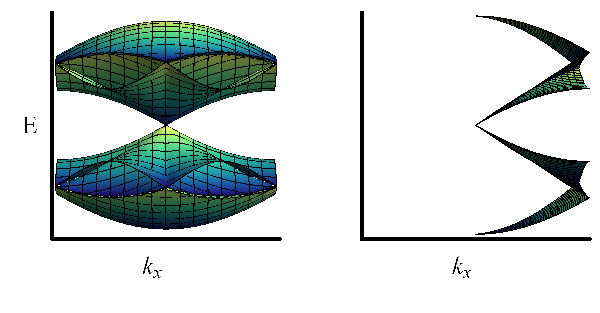
\includegraphics{Figs_Kekule/ZoneFolded.pdf}
	\end{center}
	\caption[Surface plots of the folded electronic dispersion of the Kekul\'e lattice]{\label{fig:kek:zfdisp}
		Surface plots of the folded electronic dispersion of the Kekul\'e lattice including all six energy bands.
		In the left plot the surfaces are plotted for the full Kekul\'e BZ whereas in the right plot only the symmetry reduced area is plotted.
	}
\end{figure}

\subsection{Altered hoppings}
The excitation of the Kekul\'e phonon mode does more than just enlarge the unit cell, it also modifies the hopping energies.
This is similar to the case of strained graphene where the altered bond lengths caused altered hopping energies and generated new physics.
In this case, however, the bond lengths vary with a much higher spatial frequency and the slowly varying approximation described in Appendix \ref{chap:idep} is not applicable.
In fact, the atomic displacements in Equation \ref{eq:kek:displacements} will lead to hopping alterations with a spatial frequency of $\bm{G}=\bm{K}-\bm{K'}$.
As mentioned in Appendix \ref{chap:idep}, a distortion with this frequency is expected to couple the inequivalent $\bm{K}$ and $\bm{K'}$ points.
This coupling will generate a band gap at the $\Gamma$ point of the zone folded dispersion.

Before determining the hopping alterations the bond length changes must be found.
Although it was helpful in finding the lengths of the strained nearest neighbor vectors in Section \ref{sub:PVP:straindistances}, the Cauchy-Born rule cannot be used here.
The iTO phonon causes the atoms in the A and B sub-lattices to rotate in opposite directions, an effect which an not be captured in the Cauchy-Born frame work.
Instead, the bond lengths must be calculated directly from the displacements.
Iadecola \textit{et al.} showed that the bond length alterations generate hopping alterations,
\begin{align}
	\delta t_{m,j}&=\frac{1}{3} \Delta(t) e^{i \bm{K} \cdot \vec{\delta}_j} e^{i \bm{G} \cdot \vec{r}_{m}}+\text{c.c.} \nonumber \\
	& \text{with } \Delta(t)=-i 3 \beta t_0 \frac{c^*}{a} e^{i \omega t} \label{eq:kek:hopps} \ ,
\end{align}
which have a spatial frequency component of $\bm{G}$ that couples the Dirac points \cite{Iadecola2013}.
Here $\vec{r}_{m}$ is the position of the A sub-lattice atom involved in the hopping.
Index $m$ indicates which of the three intrinsic unit cells embedded in the enlarged Kekul\'e unit cell the atom is in.
The B sub-lattice atom is specified through $\vec{\delta}_j$, the unperturbed nearest neighbor vector which connects the A sub-lattice atom to the B sub-lattice atom.
Figure \ref{fig:kek:hoppings} summarizes these indices.
For completeness, the calculation of Equation \ref{eq:kek:hopps} is included in Appendix \ref{chap:hopps}.

\subsection{Tight binding of the expanded Kekul\'e lattice}

The Kekul\'e mode causes the hopping energies in Equation \ref{eq:kek:Hreal} to be bond and time specific.
Taking $t=t_0+\delta t_{m,j}$ with $\delta t_{m,j}$ defined in equation \ref{eq:kek:hopps} breaks Equation \ref{eq:kek:Hreal} into two pieces.
The first, corresponding to $t_0$, is just the zone folding Hamiltonian in Equation \ref{eq:kek:Hzonefold}.
The second is the perturbation which opens the band gap.

Similar to the individual terms in $H_0$, each term in the perturbed Hamiltonian, $H'$, can be simplified by writing the operators in Fourier using Equation \ref{eq:kek:FT} 
\begin{align*}
	-  \delta t_{m,j} \sum_{l} \rl{m}{l}{m'}{l'} &= 
	    -\frac{\delta t_{m,j}}{N}\sum_l \sum_{\vec{k},\vec{k}'} \rl{m}{\vec{k}}{m'}{\vec{k}'} 
	    e^{i \vec{R}_l \cdot (\vec{k}-\vec{k}')} e^{i(\vec{R}_l-\vec{R}_l')\cdot \vec{k}'} \\
	    &=- \sum_{\vec{k}} \rl{m}{\vec{k}}{m'}{\vec{k}} 
	    	\underbrace{ \delta t_{m,j}  e^{i(\vec{R}_l-\vec{R}_l')\cdot \vec{k}}}_{g_{m,j,l-l'}} \ .
\end{align*}
In addition to the $l$ independent distance between involved Kekul\'e unit cells, each term depends on $m$ which indicates the old, two atom unit cell which the A sub-lattice atom occupies, and $j$ which indicates which $\vec{\delta}_j$ the hopping is along.
The associated vectors are $\vec{R}_l-\vec{R}_l' \in \{ 0, \vec{A}_+, \vec{A}_+ +\vec{A}_-,\vec{A}_- \}$ and $\vec{r}_m \in \{ 0, \vec{a}_+,\vec{a}_- \}$.

The perturbed Hamiltonian can then be constructed using Figure \ref{fig:kek:hoppings}, 
\begin{equation*}
	H'=-\frac{1}{3} \sum_{\vec{k}} \psi^{\dagger} 
	\left(\begin{array}{cccccc}
		0           & 0                     & 0                    & g_{1,1,0}        & g_{1,2,0}          & g_{1,3,0} \\
		0           & 0                     & 0                    & g_{2,3,\uparrow} & g_{2,1,0}          & g_{2,2,\rightarrow} \\
		0           & 0                     & 0                    & g_{3,2,\uparrow} & g_{3,3,\leftarrow} & g_{3,1,0} \\
		g_{1,1,0}^* & g_{2,3,\uparrow}^*    & g_{3,2,\uparrow}^*   & 0            & 0              & 0 \\
		g_{1,2,0}^* & g_{2,1,0}^*           & g_{3,3,\leftarrow}^* & 0            & 0              & 0 \\
		g_{1,3,0}^* & g_{2,2,\rightarrow}^* & g_{3,1,0}^*          & 0            & 0              & 0 
	\end{array}\right)
	\psi \ .
\end{equation*}
Using the Born-Oppenheimer approximation the electronic dispersion of the total Hamiltonian, $H=H_0+H'$, can now be calculated at any snapshot in time.
In this approximation it turns out that the dispersion is time independent.
Figure \ref{fig:kek:gapped} shows the electronic dispersion along the $\Gamma$ to $M'$ direction for a lattice distortion of $c^*/a=1\%$.
It is clear that the modified hoppings which couples the $\bm{K}$ point to the $\bm{K'}$ point opens a band gap at the charge neutrality point.
The gap has a width of $2 |\Delta|$ where $\Delta$ is given in Equation \ref{eq:kek:hopps}.
The inner two bands are gapped equally, maintaining there degeneracy at the $\Gamma$ point.

\begin{figure}
	\begin{center}
	\includegraphics{Figs_Kekule/gapped.pdf}
	\end{center}
	\caption[Gapped electronic dispersion of the Kekul\'e lattice]{\label{fig:kek:gapped}
		The electronic dispersion of the Kekul\'e lattice along the $\Gamma$ to $M'$ direction for a lattice distortion of $c^*/a=1\%$.
		The plot on the right focuses on the 310 meV energy gap at the $\Gamma$ point.
	}
\end{figure}

The generation of the band gap is not an artifact of the Born-Oppenheimer approximation.
Iadecola and coworkers solved the time dependent Hamiltonian in the low energy limit by absorbing the time dependence of $\Delta$ in a pseudo spin rotation.
The resulting Hamiltonian has the same time independent band gap of $2 |\Delta|$.
The electronic response and system bath coupling are both conserved by this rotation ensuring that the gap could be measured in an electrical transport experiment \cite{Iadecola2013}.
They were additionally able to use this fairly simple system to gain insight into the Floquet formalism used to study more difficult driven solid state systems \cite{Iadecola2013a}.

The origins of this gapped phase are very similar to the origin of the band gap in polyacetylene.
The system is continuously dimerized necessitating an expanded unit cell.
Expanding the unit cell requires a shrinking of the BZ and a zone folding of the dispersion.
Finally, the lattice modifications induce couplings which open a band gap.
The only difference with polyacetylene is that the gap in graphene does not form spontaneously.
Instead, phonons must be continuously created to gap the system.

\section{Experimental design}
\subsection{Phonon excitation}

\subsection{Band gap measurements}
From the low energy electronic dispersion the density of electronic states can be calculated.
After taking account of the two fold spin and two fold valley degeneracy, the density of states of the two dimensional electron gas is
\begin{equation*}
	\rho(\epsilon)=\frac{2}{\pi} \left( \frac{\hbar v_f}{L} \right)^2 \epsilon \ ,
\end{equation*}
where $L^2$ is the area of the graphene and $\epsilon$ the energy measured from the Dirac points.
The number of states at a given energy depends on the circumference of the Dirac cone at that energy resulting in a linear energy dependence.
Using the density of states the chemical potential can be calculated in standard graphene transport experiments.

Graphene's two dimensional nature makes it simple to continuously modify the chemical potential.
Rather than varying the concentration of a dopant as must be done for most three dimensional systems, graphene only requires the application of a back gate voltage.
A standard graphene gated field effect device is shown in Figure \ref{fig:kek:FET}.
Changing the back gate voltage ($V_{BG}$) charges the graphene-backgate capacitor, introducing charges into the system.
The differential increase in the number of charges is $dQ=C(\mu) dV$ where the capacitance is defined as
\begin{equation*}
	C=\frac{d N}{d \mu} \ .
\end{equation*}
Here $N$ is the number of electrons in the graphene and $\mu$ is the chemical potential.
For intrinsic graphene the capacitance is continuous and the total number of charges is just $N=CV/e$.
The gated graphene device shown in Figure \ref{fig:kek:FET} can be treated as a parallel plate capacitor with a plate separation of 285 nm and the dielectric constant of silicon dioxide.
Matching the integrated density of states to the number of charges in the system relates the applied gate voltage to different measurements of the chemical potential in the system.
Some useful relationships are:
\begin{align*}
	n(cm^{-2})&\sim 7 \times 10^{10} V_{BG} (Volts) \\
	\mu(meV) &\sim 30 \sqrt{V_{BG} (Volts)} \\
	\mu(meV) &\sim 1 \times 10^{-7} \sqrt{n(cm^{-2})}
\end{align*}

\begin{figure}
	\begin{center}
	\newcommand{\FEThw}{4 cm}			% Width--1 cm=1 um
\newcommand{\FETsiot}{.3 cm}		% SiO2 thickness
\newcommand{\FETsit}{.7 cm}			% Si thickness
\newcommand{\FETaut}{0.06 cm}		% Au thickness
\newcommand{\FETauw}{2 cm}			% Separation and width of the gold pad
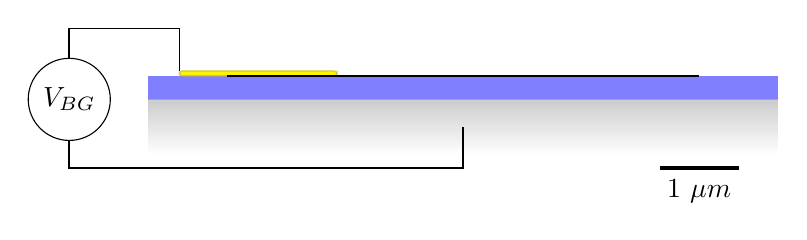
\begin{tikzpicture}[scale=1,
	sio2/.style={fill=blue!50!white,draw=none},
	si/.style={top color=black!20!white, bottom color=white},
	siedge/.style={draw=black!35!white},
	au/.style={fill=yellow,draw=black!20!yellow,rounded corners=1 pt},
	wire/.style={semithick}]
	
	%The SiO2
	\filldraw[sio2] (-\FEThw,0) rectangle (\FEThw,\FETsiot);

	%The Si
	\shade[si] (-\FEThw,-\FETsit) rectangle (\FEThw,0);
	\draw[siedge] (-\FEThw,0) -- (\FEThw,0);

	%The Gold contacts
	\filldraw[au] (-\FEThw*.9,\FETsiot) rectangle +(\FETauw,\FETaut);
	
	%The Graphene on the top
	\draw[semithick] (-3*\FEThw/4,\FETsiot) -- (3*\FEThw/4,\FETsiot);

	%The wires connecting the gate etc.
	\node (VBG) at (-1.25*\FEThw,0) [circle,draw=black]{$V_{BG}$};
	\draw[wire]  (VBG.north) -- (-1.25*\FEThw,2.5*\FETsiot+2.5*\FETaut) -- (-\FEThw*.9,2.5*\FETsiot+2.5*\FETaut) -- (-\FEThw*.	9,\FETsiot+\FETaut);
	\draw[wire]  (VBG.south) -- (-1.25*\FEThw,-1.25*\FETsit) -- (0,-1.25*\FETsit) -- (0,-.5*\FETsit);

	%Scale bar
	\draw[draw=black,ultra thick,xshift=.75*\FEThw, yshift=-\FETsit*1.25] (-.5 cm,0) -- node[anchor=north] {$1 \ \mu m$}(.5 cm, 0);

\end{tikzpicture}
	\end{center}
	\caption[Side view of a back gated graphene device.]{\label{fig:kek:FET} Side view of a back gated graphene device.  The graphene is on top of 285 nm of thermal oxide grown on heavily doped Si. }	
\end{figure}
